\documentclass[oneside]{book}

% Order packages in each section in alphabetic order
% Added some generally useful packages 
% At the end of the project, remove not needed ones

% General packages
\usepackage[english]{babel}
\usepackage{hyperref}
\usepackage[utf8]{inputenc}

%Zotero Bibliography
\usepackage{apacite}
\addbibresource{bibliography.bib}

% Layout and formatting packages
\usepackage[ruled,vlined]{algorithm2e}
\usepackage[toc, page]{appendix}
\usepackage[font=small,labelfont=bf]{caption}
\usepackage{fancyhdr}
\usepackage{float}
\usepackage[T1]{fontenc}
\usepackage[a4paper, total={6in, 8in}]{geometry}
\usepackage{listings}
\usepackage{makecell}
\usepackage{multicol}
\usepackage{soul}
\usepackage{textcomp}
\usepackage{wrapfig}
\usepackage{xcolor}

% Math packages
\usepackage{amsfonts}
\usepackage{amsmath}
\usepackage{dsfont}
\usepackage{mathtools}

% Some general page settings from 
% https://github.com/giacThePhantom/MolecularPhysics
\pagestyle{fancy}
\fancyhf{}
\lhead{\rightmark}
\cfoot{\leftmark}
\rfoot{\thepage}

\setcounter{secnumdepth}{5}

\lstset{
    frame=tb, % draw a frame at the top and bottom of the code block
    tabsize=4, % tab space width
    showstringspaces=false, % don't mark spaces in strings
    numbers=none, % display line numbers on the left
    commentstyle=\color{green}, % comment color
    keywordstyle=\color{red}, % keyword color
    stringstyle=\color{blue}, % string color
    breaklines=true,
    postbreak=\mbox{\textcolor{green}{$\hookrightarrow$}\space}
}
  % Place all packages in the prefix file

% Set up document info
\title{\Huge\textbf{Network Based Data Analysis - Lauria}}
\author{
  authorName \\
  \small telegram: \href{telegramLink}{@authorName} \\[3pt]
\small Github: \href{mainRepoLink}{mainRepoLink}}


% File structure to expand
% Files should be named #section #chapter chapterName
\begin{document}
\maketitle
\tableofcontents
  
  \chapter*{Background requirements} 
\addcontentsline{toc}{chapter}{Background requirements}

  \section*{Molecular biology background}
    It is assumed that you posses some amount of knowledge regarding the following topics:
    \begin{itemize}
      \item Molecular biology of the cell (cell types and characteristics)
      \item Molecular components of the cell (mainly proteins and nucleic acids)
    \end{itemize}

  \section*{Study design background}
    Some basic knowledge regarding cell lines, immortalized cell lines, model organisms, human studies and their pros and cons are required. \textit{This section might be expanded more clearly in the future}.

    %TODO Decide if actually expanding it or not


  \part{Introduction to omics}

    \graphicspath{{chapters/images/01/}}
%TODO Fix image sizes, captions and references 

\chapter{High-throughput biological data}
  High-throughput techniques, ofter referred to as \textbf{omic techniques}, are a way to collect extensive, comprehensive, quantitative and large scale data on a certain aspect of a biological system. The main omics data types are genomics, transcriptomics, proteomics, metabolomics; each of them possesses specific individual technologies and methods. 

  \section{Required biological background}
    It is assumed that you posses some amount of knowledge regarding the following topics:
    \begin{itemize}
      \item Molecular biology of the cell (cell types and characteristics)
      \item Molecular components of the cell (mainly proteins and nucleic acids)
    \end{itemize}

  \section{Genomics}
    \textbf{Genomics} refers to the study of the genome, which is the entire DNA (or RNA in some bacteria and viruses) content of a cell. The focus is generally on the variation of the genome of an individual (or a group of individuals) compared to a reference genome (a sequence that is shared by most individuals of a scpecies). Particularly important is the study of \textbf{SNPs} (Single Nucleotide Polymorphisms) which allows to retrieve information such as philogenetics, disease predisposition, forensic applications (individual recognition, paternity testing...) and many others. SNPs can be studied either via \textbf{DNA microarrays}, which are economic since they target only specific regions of the genome where the presence of SNPs is known, or via \textbf{whole genome sequencing}, which is more expensive but gives information. 
    
    \subsection{Genomic wide association studies}
      \textbf{Genome Wide Association Studies} (GWAS) are studies where many genetic markers are studied across the genome a population in orded to try and correlate them to specific conditions (mainly predisposition and presence of disease).

      \begin{figure}[h]
      \caption{Manhattan plot: Mahnattan plots are a common way to represent GWAS results}
      \centering
      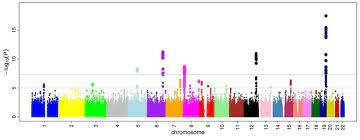
\includegraphics[width=0.6\textwidth]{ManhattanPlot.jpg}
      \end{figure}


  \section{Transcriptomics}
    The \textbf{transcriptome} is the collection of mRNA species/transcripts in a cell at a given time. It can provide a lot of information on cell state, growth conditions and many others, which is why it is heavily studied; moreover transcriptomics is \textbf{robust}, relatively \textbf{cost effective} and \textbf{user friendly}.
    
    \subsection{Microarrays}
      \textbf{Microarrays} can be used to measure levels of mRNA in a high-throughput fashion.
      Roughly, a microarry workflow can be summarized as:
      \begin{itemize}
        \item Extract RNA content from cells
        \item Obtain fluorescence-marked cDNA
        \item Hybridize the cDNA with the DNA probes on the chip 
        \item Wash chip to remove non-hybridized cDNA
        \item Record output fluorescent signal
        \item Normalize the result:
        \begin{itemize}
          \item If using a 2 color microarray (red-marked test sample, green marked control sample), you obtain the fold expression of the transcript compared to the reference (red = overexpressed, yellow = same expression level, green = underexpressed)
          \item If using a single color microarray (only marked test sample) the output can be normalized in various ways, generally substracting the signal of aspecific probes (of the 20-25 bases a couple of them are mismatched, to test for aspecific interaction)
        \end{itemize}
        Further normalization steps may be required
        % \cite{smythNormalizationCDNAMicroarray2003}
        \item Analyze the output
      \end{itemize}

      \begin{figure}[h]
      \caption{Microarray output: Genes with different expressions can be visualized, each column is a sample and each row is one of the 25 genes. The colour represents the level of expression}
      \centering
      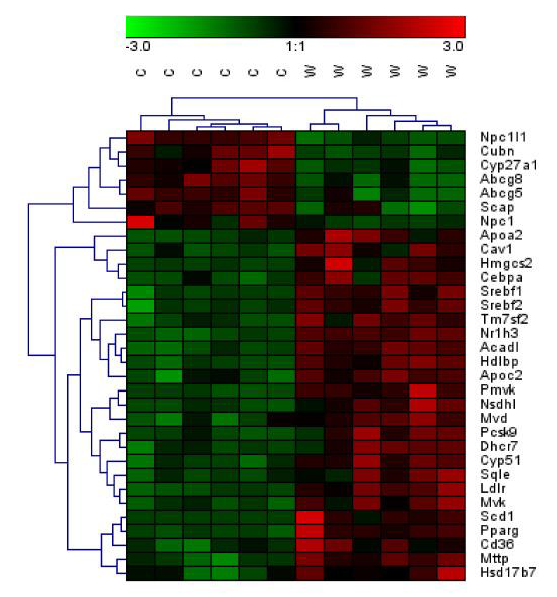
\includegraphics[width=0.6\textwidth]{MicroRNAresults.PNG}
      \end{figure}

    \subsection{Next generation sequencing}
      \textbf{Next generation sequencing} (NGS) is another way to analyize the transcriptome; each mRNA species in each sample is broken into fragments, and all fragments are sequenced base by base. The current technologies manage to sequence small pieces of RNA, around 250 bases. By using overlapping ends of the fragments, we can reassamble RNAs. A higher amount of fragments grants an higher coverage. This method allows \textbf{massively parallel sequencing}, \textbf{sequencing of both known and unknown transcipt} (no probe requirement), detecting transcripts in a \textbf{high dynamic range} (up to $10^6$ copies)

      \begin{figure}[h]
      \caption{NGS flowchart}
      \centering
      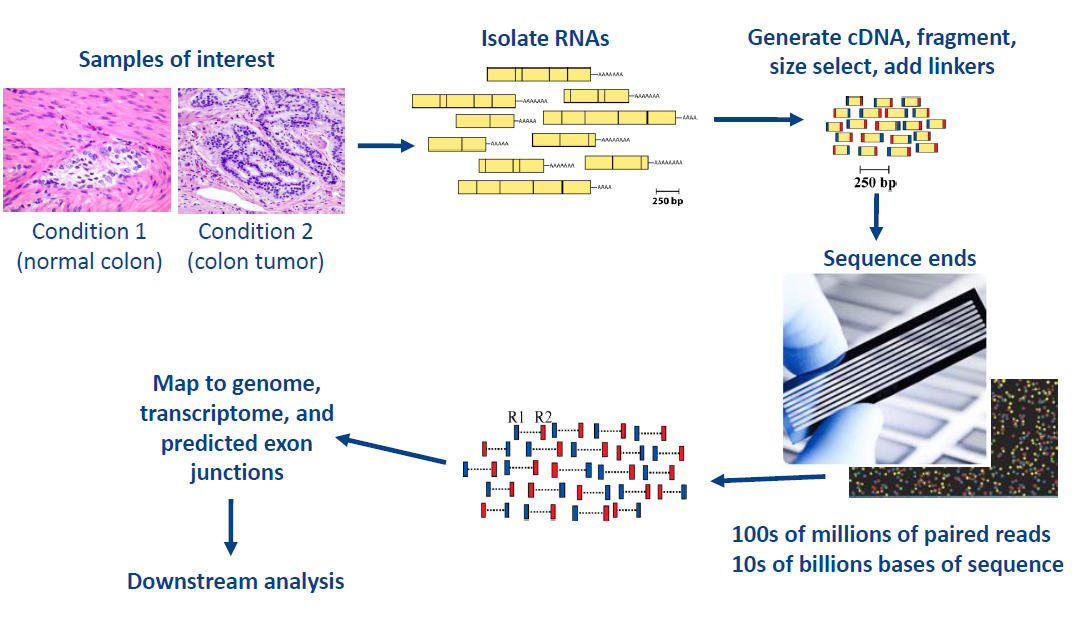
\includegraphics[width=0.6\textwidth]{TranscriptomicsNextGenSeq.PNG}
      \end{figure}

    \subsection{RNA-seq pipeline}
      After obtaining the raw sequencing results, the RNA-seq pipeline uses some other resources, namely input files (reference genome, gene annotation) and programmes (some accessed through cloud to speed up data analysis), to obtain polished information and results.

      \begin{figure}[h]
      \caption{RNA-seq pipeline}
      \centering
      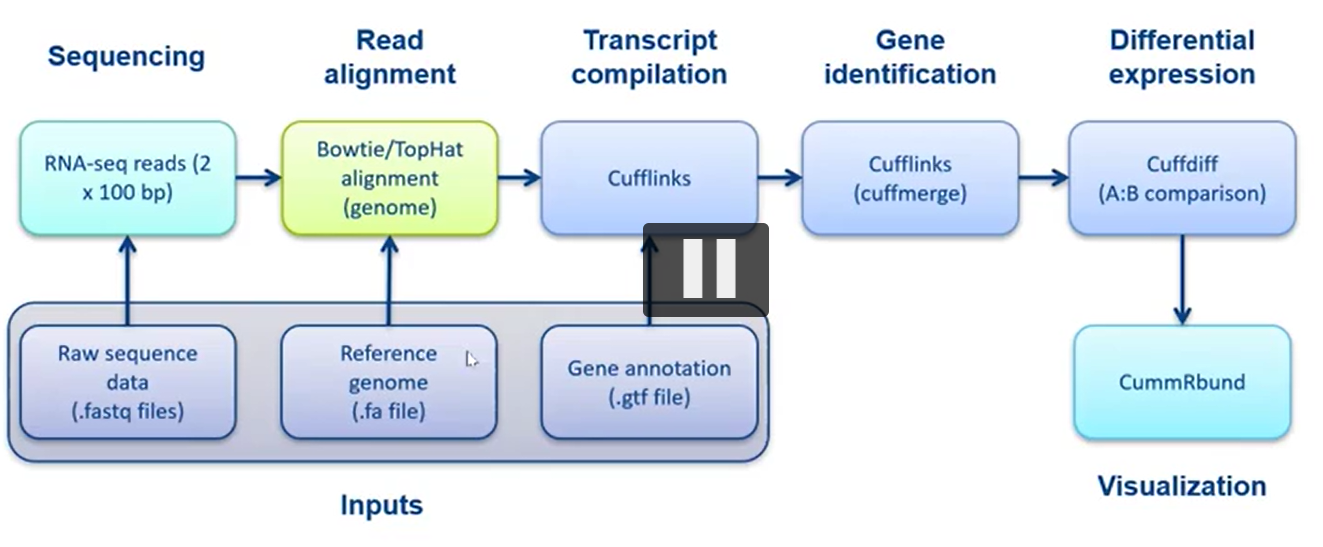
\includegraphics[width=0.6\textwidth]{RNAseqpipeline.PNG}
      \end{figure}

    \subsection{Microarrays vs sequencing}
      Overall, microarrays are more economic but can only give information on transcripts for which a specific probe exists on the chip. They allow to obtain differential expression studies but not absolute quantification. Sequencing is more costly, but unbiased and higher-throughput; moreover it allows further analysis, such as mapping and absolute quantification.

  \section{Proteomics}
    The \textbf{proteome} is the set of all proteins produced under a given set of conditions. The analysis of the proteome, called proteomics, has countless applications. Proteomic techniques allow for high-throughput analysis of protein content, yet again the throughput is significantly lower than transcriptomic techiques: this is because proteins are more complex than nucleic acids, both in structure and sequence, and they do not have a convenient 1:1 pairing pattern. For this reasons, proteomic techniques usually rely on other physical characteristics, mainly \textbf{mass} and \textbf{charge}.

    \subsection{2D gel electrophoresis}
      Standard gel electrophoresis separates proteins based on their size (varying the crosslinking rate of the polyacrylamide net); this method has very limited resolution (it is influenced by many factors, such as denaturation, SDS coating, fragmentation...).
      2D gel electrophoresys partially increments the resolution since it separate proteins based on both weight and charge.
      The standard protocol for 2D gel electrophoresis consists of:
      \begin{itemize}
        \item Protein extraction, purification and usually denaturation
        \item First dimension electrophoresis: proteins migrate in a low density gel in which molecules have been placed to create a pH gradient. The proteins distribute along the gradient solely because of their charge (regardless of mass)
        \item Second dimension electrophoresis: the first dimension gel is placed at the edge of a regular polyacrylamide gradient gel, which allows to separate the molecules by weight. 
        \item Coloration and acquisition of gel signal
        \item The result is a sort of map, with increasing pH value from left to right and decreasing weight from top to bottom.
      \end{itemize}
      These maps can be then compared either with maps from other samples (to identify differences) or with databases to identify the proteins spots. Notice that this procedure does not technically identify univocally the protein and thus, if required, you might have to cut the protein spot from the gel and procede with further analysis. Another significant problem with this technique is the need for large amounts of samples to have significant signal levels.

      \begin{figure}[h]
      \caption{Isoelectric focusing: separation of proteins in a pH gradient}
      \centering
      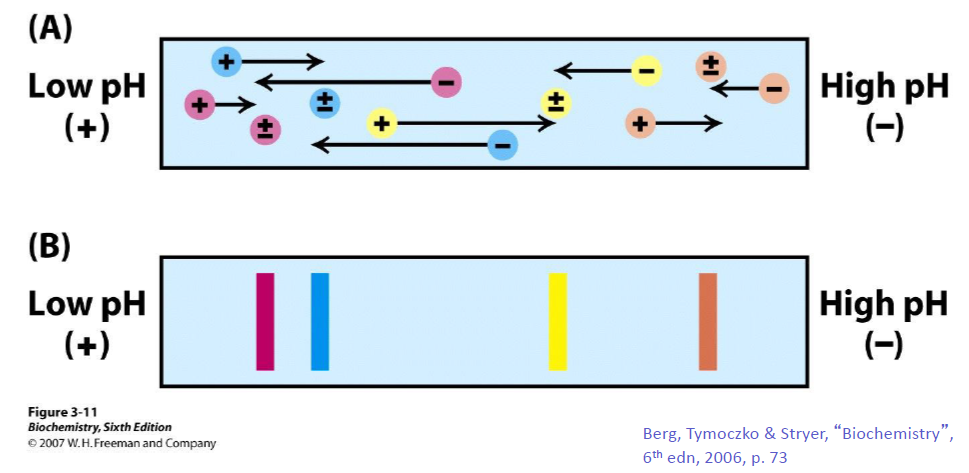
\includegraphics[width=0.6\textwidth]{IsoelectricProteinSeparation}
      \end{figure}

    \subsection{Liquid chromatography/mass spectrometry}
      Mass spectrometry consists of a plethora of techniques that allow to separate molecules based on their mass to electrical charge ratio. This technique allows for high-throughput identification of proteins (without need for further analysis). The main limitation of mass spectrometry is the need for highly purified protein extracts (and thus labour intensive procedures) since it is highly susceptible to contaminants; for this reason the protein extract is usually purified and diluted using liquid chromatography and the output is analyzed via mass spectrometry (from which the name liquid chromatography/mass spectrometry or LC-MS for short). Another big advantage of this technique is the very low amount of sample required (some $\mu g$ of purified proteins are enough). Mass spectrometry does not allow for absolute quantification but only relative quantification (due to peptide volatilization and other factors). LC-MS can usually identify up to about 1000 proteins per sample (more realistically around 600-700 due to dynamic range issues). LC-MS can be used to study also post-traslation modifications (such as phosphorilation).

    \subsection{Protein arrays}
      \textbf{Protein arrays} are conceptually similar to DNA arrays, but instead of DNA probes they use \textbf{aptamers}, which are oligonucleotides or peptide molecules designed to uniquely bind to a specific molecule. Proteins bind the aptamers and a fluorescent signal is used for detection. This method is easy and cheap, but it measures a low amount of proteins and only proteins for which an aptamer was found. It is still an emergent technology.
      % \cite{neaguProteinMicroarrayTechnology2019}.

      \begin{figure}[h]
      \caption{Protein array}
      \centering
      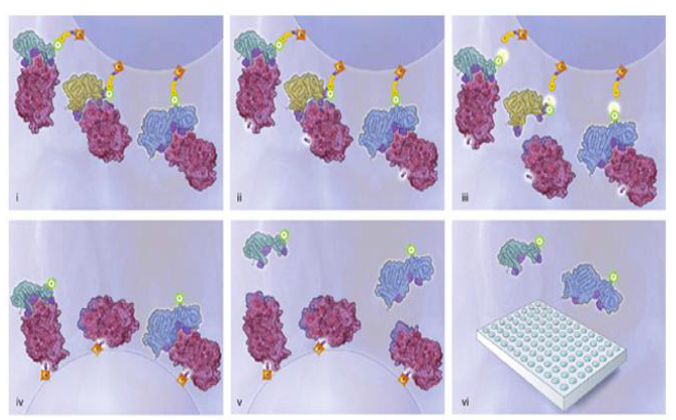
\includegraphics[width=0.6\textwidth]{ProteinArray}
      \end{figure}
    
    \subsection{Proteomics vs transcriptomics}
      Both proteomics and transcriptomics are very powerful techniques. In general transcriptomics is cheaper, more robust and user-friendly, while proteomics pose some more limitations, namely due to protein purification and stability. Both techniques keep being developed since they provide different informations, for example transcriptomics allows to study non-coding RNAs while proteomics allows to study post-translational modifications (the opposite in not true).

  \section{Metabolomics} 

    \textbf{Metabolomics} is a field of life science research that uses high-throughput technologies to identify and/or characterize all the small molecules or metabolites in a given cell, tissue or organism (the so called metabolome). There are two main approaches in metabolomics:
    \begin{itemize}
      \item Quantitative methods: quantitatively identify target metabolites in a sample
      \item Chemometric methods: profiling samples based on metabolites in them
    \end{itemize}
    These approaches can be useful, for instance, to early detection and diagnosis of diseases, since certain metabolites correlate do higher risk of certain pathologies.
  
  \section{Other high-throughput data sources}
    Countless other sources of high-throughput data exist and many more are becoming viable. 

    \subsection{Microbiome}
      With the term \textbf{microbiome} we collectively refer to all the microbes in the human body, whether they are bacteria, fungi, protozoa, viruses or other. This heterogeneous population is of interested since it is highly represented in most regions of our body; the role of microbes is important since they contribute to some physiological functions of the organism (gut microbes), they can cause pathologies when deregulated, their populations show differences among individual hosts.
      (\textit{To go into more detail, please refer to the "Computational Microbial Genomics Notes - Segata" available \href{https://github.com/giacThePhantom/computational-microbial-genomics}{\textbf{here}}})

    \subsection{Epigenomics}
      \textbf{Epigenetics} is the study of heritable changes in gene activity that are not caused by changes in the DNA sequence. Some mechanisms that produce such changes are \textbf{DNA methylation} and \textbf{histone modification}. Both mechanisms alter how genes are expressed without altering the underlying DNA sequence.
      %TODO potentially add more

      \begin{figure}[h]
      \caption{Examples of epigenetic modifications}
      \centering
      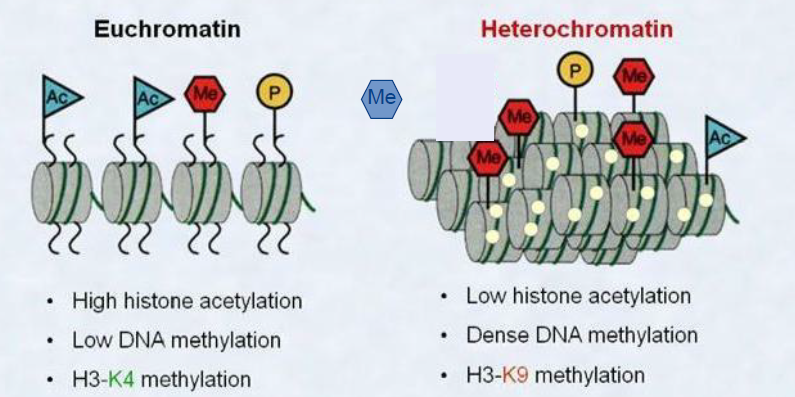
\includegraphics[width=0.6\textwidth]{EuEteroChromatin}
      \end{figure}

    \subsection{Micro RNAs}
      Micro RNAs, or miRNAs, are a family (around 1000 in humans) of short (20-22 bases) non-coding RNAs which affect mRNA translation and therefore protein expression. They are produced as precursors in the nucleus, then when they find and pair with their target sequence, they recruit cellular machinery that activates them and causes transcript degradation. miRNAs can be isolated from total RNA and can be profiled to get information on genes that are currently regulated.
      %TODO potentially add more

    \subsection{Interactome}
      The \textbf{interactome} of a protein is the set of molecules (generally other proteins) that interact with that specific protein (therefore we usually talk about protein-protein interaction). Studying the interactome of a protein can help understand its function and possible ways to modulate its activity. There are databases for interactomes. Interactomes are generally shown in 3D graphs, with nodes representing proteins and lines representing connections between them.  
      %TODO potentially add more

\chapter{Clinical trial study design}
  
  \section{Required background}
    Some basic knowledge regarding cell lines, immortalized cell lines, model organisms, human studies and their pros and cons are required. \textit{This section might be expanded more clearly in the future}.

    %TODO Decide if actually expanding it or not

    \graphicspath{{chapters/images/02/}}

\chapter{Working with transcriptomics}

  \section{Measuring RNAs and proteins}
    There are several ways to measure proteins (western blot, ELISA, northern blot, enzymatic assay) and RNAs (microarray, RT-PCR, RNA-Seq). Protein and mRNA levels often do not correlate (or only loosely); for this reason, studying directly the protein levels would be the best option. Yet again, due to the fact that there are no high throughput methods for absolute protein quantification, no genome-wide protein arrays and the fact that protein sequencing is difficult, more often then not mRNA levels are still used. The two main approaches for transcript measurement are DNA microarrays and RNA-seq. 

  \section{DNA microarrays}
    For microarray protocol see previous chapter.
    % TODO Add reference

    \subsection{Most common microarrays}
      DNA microarrays are the older technology for RNA quantification (started in the early '90s). Early microarrays were glass slides with probes spotted by the individual laboratories, then companies started producing more refined versions. One of the most used devices is the \textbf{Affymetrix GeneChip}, capable of analyzing all the genes of an organism (available for different species), with multiple oligonucleotide-probes per transcript, with control mismatch sequences. It allows to analyze one sample at a time and to obtain an absolute quantification of the transcript levels (more or less). Another common technology is \textbf{Illumina BeadChip}, in which the probes are spotted on beads placed in wells. Compared to Affymetrix GeneChip, Illumina BeadChip has higher throughput and allows the use of two fluorescent molecules at the same time.
    
    \subsection{Microarrays advantages}
      Microarrays allow to quantify not only mRNAs, but also miRNAs, SNPs and others. They allow to study all the genes in the genome, including the splicing variants, and they are reliable for gene expression quantifications (and comparative analysis). They are cost effective and easy to analyze, thanks to the bioinformatics resources that are now available. Microarrays give direct (non-absolute) quantification of the mRNA.

	  \begin{figure}[ht]
	  \caption{}
	  \centering
	  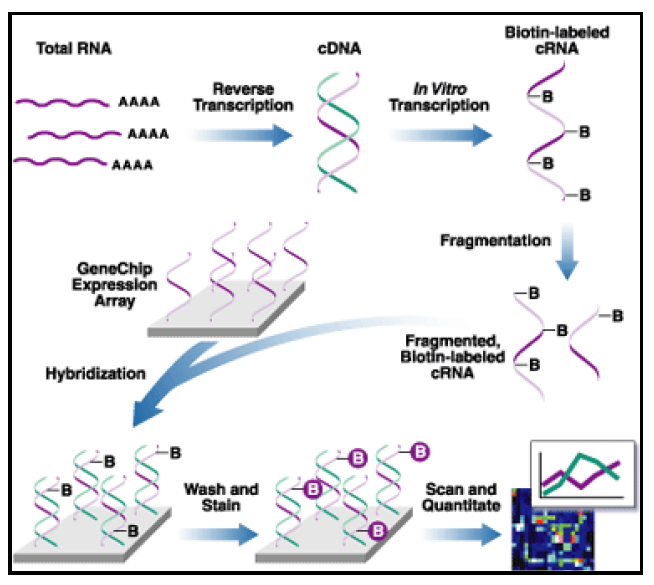
\includegraphics[width=0.6\textwidth]{microarrays}
	  \end{figure}

    \subsection{Error sources in microarrays}
      There are several possible sources of error when working with microarrays:
      \begin{itemize}
        \item RNA contamination during extraction 
        \item Poor quality, insufficient extraction or degradation of RNA
        \item Bias in which molecules are transcribed during retro transcription
        \item Bias in ligation of the fluorescent protein reporter
        \item Cross hybridization, meaning the aspecific binding to the wrong probe (especially if the sequence is long)
        \item Aspecific fluorescence and in general background noise
        \item Scanning errors during image acquisition
      \end{itemize}

	  \begin{figure}[ht]
	  \caption{}
	  \centering
	  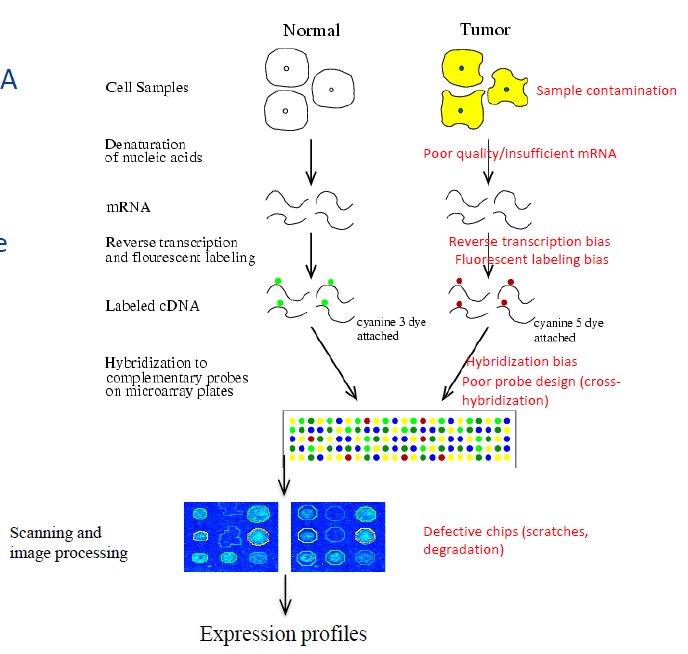
\includegraphics[width=0.6\textwidth]{ProblemsMicarrays}
	  \end{figure}

	\subsection{Noise handling and normalization in microarrays}
      Some methods exist to reduce the noise (error). For instance, the Affymetrix GeneChip uses two probes for each transcript, one with perfect match and one with a single \textbf{mismatch}; if you subtract the mismatch fluorescent from the perfect match one, you remove some of the fluorescence signal due to aspecific interactions (it is not the most efficient correction). Moreover Affimetrix GeneChips come with quality control checks data. 
      Another way to remove noise is \textbf{Robust Multi-array Average (RMA)} which is an algorithm that takes into account the fluorescence levels of the entire chip and applies a correction. 
      \textbf{Spy probes} are basically control probes, meaning that they should not show any sign of fluorescence; these probes are useful to detect contaminations (for instance you can use mouse-RNA probes on human-RNA chips).

      In order to obtain an absolute quantification of the transcript levels, other steps are required in addition to noise correction; these steps are generally referred to as normalization. These steps make use of statistical tools, control genes and others to correct for chip, probe, spatial, intra and inter chip variation.

    \subsection{Other problems with microarrays}
      Further problems regarding microarrays can be found:
      \begin{itemize}
		\item A certain transcription level (detection limit) is required to have a signal
		\item To quantify a transcript, a probe for it must be present on the chip (therefore you cannot study unknow transcripts)
		\item Most chips cannot differentiate splicing variants well (even though there are some chips that try), since usually the match is checked for a subset of the sequence 
		\item Chips cannot differentiate RNA synthesis and degradation
		\item Chips do not provide information on post translational events
		\item The bioinformatic analysis may be difficult
      \end{itemize}

    \subsection{Microarray data processing}
      An Affymetrix GenexChip generates several type of files:
      \begin{itemize}
      	\item DAT (image file)
      	\item CEL (raw data file)
      	\item CDF (chip definition file)
      \end{itemize}
	  All platforms have different data formats, which can complicate the analysis.  
      \textbf{Bioconductor} is a open source software project for the analysis and comprehension of genomic data. It provides a wide range of powerful statistical and graphical tools.

	  Microarray data can be found in repositories, such as \textbf{Array express} (UK), \textbf{Gene Expression Omnibus}(founded by NIH, USA), CIBEX (JP). Notice that Array express and GEO contain non-overlapping data. \textbf{Recount3} has a smaller number of datasets, most of which already in GEO, but these datasets have already been partially processed. Other databases can be used for annotation purposes, such as NetAffx, Ensembl, TIGR and Stanford. 

      There are some microarray data standards, namely:
      \begin{itemize}
      	\item \textbf{MIAME} (Minimum annotation about a microarray experiment); this entails a comprehensive description of the experiment, therefore allowing replicates of chips, samples, treatments and settings and facilitating data comparison. It is required for most recent publications.
      	\item \textbf{MAGE-ML} (Microarray gene expression markup language). It describes both the experiment (MIAME) and the data. Tools are available for processing this format.
      \end{itemize}


  \section{RNA-Seq}

	RNA-Seq is a more recent way of measuring gene expression levels which uses next generation sequencing techniques. The idea is that, by sequencing each molecule in the sample, you are able to obtain an absolute quantification.
    
    \subsection{RNA-Seq workflow}
      A \textbf{whole transcriptome shotgun sequencing} approach is used. The general workflow can be described as follows:
      \begin{itemize}
        \item The whole RNA content of the sample is broken into fragments using restriction enzymes; this is repeated for multiple samples with different restriction enzymes in order to have different breaking points (and thus facilitating following steps since it increases the amount of overlapping segments).
        \item RT-PCR is performed in order to obtain cDNA from all fragments. Each cDNA fragment is sequenced and the results are called \textbf{raw reads}, which are store in a fastQ file, which is a text-file where each row is a sequence (produced by Illumina sequencing machines).
        \item Quality control is performed on the reads (sequence quality, GC content, presence of adaptors, overrepresented K-mers, duplicated reads). After quality control and adaptor sequence trimming you obtain the \textbf{reads}.
        \item The reads are then re-assembled and mapped against a reference sequence (genome for splicing information, transcriptome for faster computation) in order to obtain the original sequences present in the sample. This step requires a computer with a lot of ram and storage, way more than the average laptop; cloud computing is a way to solve this problem. The output is generally stored in a BAM file, which is a text-file with each read and next to it the coordinates with reference to the genome.
        \item After mapping, the number of reads for each sequence is computed; those integer numbers are called \textbf{raw counts} and are stored in a count matrix where each row is a gene, and each column a sample, each cell is the number of counts for that gene in that sample. The database recount3 provides count matrices from some RNA-Seq experiments.  
        \item Pre-processing refers to a series of steps used to remove bias and normalize your data (inter and intrea sample normalization, normalize for gene lenght, normalize for number of reads per sample); the output are the \textbf{counts}, 
        \item Counts can be used for several types of analyses, such as differential expression analysis, functional analysis, network-based enrichment analysis.
      \end{itemize}
      %TODO Add image
    
    \subsection{RNA-Seq data normalization}
      Several normalization algorithms are available, both for within-sample normalization and for between-sample normalization (for instance if you want to perform t-test on differential gene expression); some of them are shown in the tables below.
      %TODO Add reference images
      Notice that sometimes the order of the normalization steps actually matters (TPM is slightly better than RPKM for instance).


  \part{Introduction to PCA}

    \graphicspath{{chapters/images/03/}}

\chapter{Introduction to principal component analysis}

	\section{General strategy to analyze a dataset}

	\section{Principal Component Analysis}
	Data from a big table, Starting point is a $ p x n $ matrix with \textit{p} is equal ot the number of genes and \textit{n} to the number of samples. The number of samples has to be between 40 to 100, if smaller than 20 analysis become difficult. If bigger, it is possible to use a subset of the dataset. p is normally larger than n, as of course genes are more. Source of errors are introduced, making noise. Generally a lot of non informative data, or even wrong, most often it is necessary to transform the data and normalize it. 

	Formulate a question and try to answer to that, about the aim, which genes are differentially expressed between different groups. Is it possible to group samples with similar expression profile?. Think about the statistical test then. Once done the question, open data file, data normalization, transformation and PCA. Questions through the description of the experiment. 

	For \textbf{class comparison}, it is possible to use a \textbf{t-test}, what are the genes whose expression is different between different groups. Statisticall significance has to be detected. T-test to understand if $H_0$ is true or the alternative hypothesys is True. The test gives a \textit{p}-value.
	Calculate the $T_{observed}$. Difference obtained by chance or not? Are the data extracted from the same distribution (in this case mean of the two groups should be similar)? 
	A solution is to use a correction method, like Bonferroni. The problem of \textbf{threshold} is not already solved, normally $0.05\%$. The percentage remains arbitrary. $0.05$ means that you have a mistake as result only for the 5\% of the times. 
	The ones with smaller \textit{p}-value are the most interesting. It is possible to sort the genes and take those with lower values of \textit{p}-value.

	Estimates of mean and standard deviation, very different values in different experiments. Especially if number of samples is low. Larger number of samples make the estimates more robust.

	The \textbf{multiplicity problem} has to be considered.
	For a given gene and a given type I error rate ($ \alpha=5\% $), we know that this gene has a
	5\% probability to be a false positive. Thus, when doing one test at $\alpha=5\%$  for each
	gene, we know that the number of false positives will be 5\% times the number of
	tests (5 FP for 100 tests, 50 FP for 1000 tests,…, 2200 FP for 44000 tests).
	The T-test produces more reliable results with normal distributed data.


	The adjustment is made to have a new \textit{p}-value.

	It is possible to \textbf{rank} the genes based on the \textit{p}-value, those with the lowest \textit{p}-value are those more interesting. take for example the first thirty, draw a heat-map, where column is a sample and row is a gene. The t-test makes assumption on data, it is not the best oprion for class comparison. You have to set a threshold, and establish which are interesting and which not. The choice of threshold is always arbitrary. 

	It has to be started the analysis. Open the file, read the data, maybe to many $ 0s $. It is done a data normalization and a PCA, a way to reduce dimensionality of the dataset. 

	\subsection{Normalization}
	Ranges of values are presented through box-plots. The middel line is the median. Points out of whiskers are outliers. Whiskers represent 1.5 times the interquartile range %TODO .
	The range of values are really disalligned, for no reason, variation in the data that has no biological explanation. Reallign the boxes through normalization.

	The variation can be sistematic, same for all the samples, or it can be random. The best way to deal with radom is to do several replicates. Random variations have a 0 mean. 

	The sources of variation :

	Dye bias: differences in heat and light sensitivity, efficiency of
	dye incorporation
	Differences in the amount of labeled cDNA hybridized to each
	channel in a microarray experiment (here channel is used to
	refer to a particular slide/dye combination.)
	Variation across replicate slides
	Variation across hybridization conditions
	Variation in scanning conditions
	Variation among technicians doing the lab work
	etc.

	The general strategy for normalization is to use
	House keeping genes,
	considered not to change on average across samples and
	conditions. Remove residual variation of house keeping genes taking a pool of these genes.

	The simplest method: subtract the median from each values of the profile $\Rightarrow$ all the samples are alligned on  $0$, through the shifting up and down of the boxes. 

	Variants of normalization: batch effect: source of error is known, for example different processing (very unlikely the same results), some packages are available; microarray done in different days.

	Once done the alignment to 0 of the median, boxplots with the median alligned. The amplitude of the boxes is not equal, scale normalization can be done: it can be done deviding by the standard deviation for that profile for each profile, each value. To do both the normalization processes, 

	%R commands and suggests to ADD %TODO
	it can be used the \textbf{scale} built in function of R.  

	The t-test should be done on the final version of the data. 

	\textbf{\textit{MAD}} stands for "\textit{median standard deviation}". The possible presence of outliers justify the use of the median, off range, so extreme that can be produced by errors. Remove or mantain? it influences enormously the calculus of the mean and of the standard deviation. Median is not affected instead by outliers.

	Other more sufisticated methods are available to normalize the data. 

	\subsection{Data transformation}
	There has to be a reason for that.
	Replace the numerical values with $ \log $ of the values. This changes the shape distribution of the data, maybe obtaining data more normally distributed. Ranks are also usable, where each value is substitued with its position after that it is sorted from the lowest to the highest.
	Z-scores are obtained after standardization of values.

	The $ log $-transformation is made on graphs not normally distributed. T-test can be used on normal distributions, and this is considered as True when performing the test.

	\subsection{Principal component analysis (PCA}

	Also known as latent vectors, latent variates, principal axes, 
	principal factors, reduce dimensionality. \textbf{Reduce dimensionality}, each sample 30000 values collection, dataset can be seen as a series of points with 30000 dimensions. Obviously, the number of dimensions has to be reduced. PCA plots are generally 2-dimensionals or 3-dimensional.

	Given a sample of
	n observations on a vector of p variables, with p variables/dimensions equal to 30000

	\begin{equation}
	{x_1, x_2, \dots, x_n} \in  \Re^p
	\end{equation}

	it is possible to go from a space of p dimensions to a space of n dimensions. transformation from the space of the xs to the ys. 

	Using the linear regression, we are going to obtain \textit{n} coordinates transformed (transformation), where \textit{n} is equal to the number of samples. We choose the best dimension which describes the most part of the variability of our data ($ y_1 $). The second dimension has to be ortoghonal to the first one ($ y_2 $). Once we have identified those directions, the point will have new coordinates. 

	eigenvectors are arrays of n values, eigenvalue.
	we obtain the directions that we like, how much the stress also. Only 2 or 3 are representative of the variability of the data 

	each x represent a gene, ys are said metagenes, imaginary genes, whose level of expression is given by the linear combination of all the genes. 

	\begin{equation}
	y_{i,j} = a_{j,1}x_{i,1} + a_{j,2}x_{i,2} + \dots + a_{j,p}x_{i,p}
	\end{equation}

	A few metagenes are needed to describe variability of data. Which metagenes to use? Usully the first, the second and the third are used. 

	In the process $ S = B^T B $ it is the covariance matrix. If the data was standardized, correlation and covariance are the same. Correlation matrix vs covariance matrix %TODO .

	\textbf{in R...}: \textit{prcomp} is built-in into R. Array of colours to be used. one gene per row and a sample per column, in some cases, as for \textit{prcomp}, it is needed the inverse arrangement. 

	In new set of coordinates, directions should be orthogonal, the first ax should be the one over which the cloud of points is more stratched. 

	If data is a ball, data obtained by random. The way to obtain the coefficients so that it is satisfied ... is to use the covariance matrix, obtained through the multiplication of the matrix per itself transposed. Take the eigenvectors, each one is a row of that matrix, while instead the eigenvalues provide an estimate of the percentage of the variability of the corresponding axes is out of the total variance (how spread along that direction).

	The covariance matrix is symmetric and positive. As a consequence, all the eigenvalues are positive. 

	computations of eigenvalues and eigenvectors are made through a function. Coordinates of the points in the new set of coordinates as output. 

	The skree diagram make us see which components are relevant

	Scores %TODO


	\begin{figure}[h]
	\caption{Scree diagram}
	\centering
	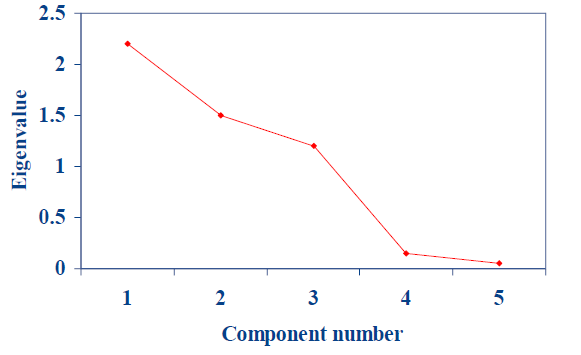
\includegraphics[width=0.6\textwidth]{skreeDiagram}
	\end{figure}


	\begin{itemize}
		\item \textbf{Inspect dataset:} check data in there, not too many NAs. 
		\item \textbf{Normalization}: The sistematic source of variation can be eliminated by using a box-plot, which means great amount of variation. normalization is made by subtracting the median.
	Align the size of the boxed by aligning the standard deviation
		\item \textbf{PCA}:
	\end{itemize}



	\subsection{Series Matrix of GEO}
	on the left column, there are present informations regarding the authors, date, platform (GEO assigns it), the type. Each line starts with !, which indicates this is a piece of metadat. The second section is specific to each sample. The third section contains the data. 





  \part{Machine learning}
    analysis:
classification: find a way to assign a label to each sample of a dataset. can provide a list of genes to perform classification. 

The classification problem was solved in different ways tries. None of the methods works best for every possible dataset. depends on the nature of the data. select the best performing one. \\

Many of the methods depend on machine learning: learn from data. Statistical tools can be used combined with machine learning. search engines, natural language processing. Medical diagnosis.\\

supervised against unsupervised learning. learning extract features using a small dataset. the algorithm can so be used to other samples. Unsupervised methods are instead used without ... %TODO\\


\section{Unsupervised learning}

data clustering, is used also as a synonym to unsupervised learning. TWo methods we will see.
it consists in understanding how info points could be clustered. Clustering among almost every field. \\
Main aspects:
\begin{itemize}
	\item \textbf{Distance function}: a way to measure similarity or dissimilarity
	\item \textbf{Clustering quality}: it has to be maximized. Intra-clusters distance could also be done.
	...
\end{itemize}

clustering algorithms could be partitional or hierarchical. 


\subsection{K-means clustering} 
it is a partitional clustering, using a distance function, it minimizes the intra-cluster distance. K is the expected number of clusters, and it has to be given to the algorithm. sometimes the number of clusters cannot be said certainly. Leads to the user the decision about the number of clusters.
Takes K seeds, which arethe initial centroids, cluster centers. Assign each node to the closest centroid. Recompute the centroids and another time it is done the process.
A reasonable criteria to stop the algorithm: no reassignment of data points to different clusters, minimum change of the centroids, minimum decrease in the SSE: when this distance goes under a threshold, the algorithm stops. 

\begin{equation}
\sum_{j=1}^k\sum_{x\in
\end{equation}

The ingredient is the distance function, the Euclidean distance in particular, application of the Pitagoran theorem.

\begin{equation}

\end{equation}

You can think about other possible methods\\\\

\begin{itemize}
\item \textbf{Strengths}: very intuitive, the complexity is ..., it is a linearly complex algorithm, it is the most popular clustering algorithm.\\
	\item \textbf{Weaknesses}: you have to know k, outliers affect the decision of the algorithm. Solution: reduce the dataset excluding the outlier. Run the algorithm different times on subsets of the dataset. It is also sensitive to the initial seed, solution: aggregate results of multiple runs. It can be used in case of simple structures, round, for difficult shapes, the algorithm doesn't work well.
\end{itemize}
	
\subsection{Outliers}
It is difficult to find a rule to identify them, it is subjective, you decide where to cut.  Interquartile range, multiply per 1.5. The 1.5 parameter can be modified, it is arbitrary, it's controversial the number usage, more robust to outliers or not. 

\subsection{Hierarchical clustering} 
it is another clustering method based on a distance matrix. It is based on a dendogram, a tree. A way of clustering raws and columns of a matrix. It can be constructed top-bottom or bottom-up. \\

The divisive clustering abd agglomerate clustering are possible.\\

each point generates a node of the tree, a cluster. merge 2 clusters at every level, 

for each node you have to compute distance with all the other nodes. The final step is to obtain the total cluster (4 in figure \ref{}). The result is the dendogram.\\

\textbf{Where are the final clusters?} depends on the level of the "cut", imagine drawing an horizontal line on the dendogram graph. \\

How to measure distance between two sets of points. 
Single link method: the distance between two clusters is the distance between two closest data points. 
Complete link method: the distance between the furthest points
Average link: a compromise
Centroid method the distance between two clusters in hte distance between their centroids. 

distance matrix needed. Due to complexity, it is hard to use for large datasets.\\

h larger than two puts more enphasys.  




  \part{Introduction to LDA}

  \part{Lasso/Ridge regression}

  \part{Rank-based signatures}

  \part{Functional enrichment analysis}

  \part{Network analysis}

\end{document}
